\documentclass{cosart-xetex}
\renewcommand{\figurename}{\bf  图}
\renewcommand{\tablename}{\bf 表}
\CTEXsetup[format+=\raggedright]{section}
\graphicspath{{fig/}}
\begin{document}
\setlength{\parskip}{1.1ex}
\setlength{\baselineskip}{1.7em}
% 使用旧式footnote符号
\renewcommand\thefootnote{\fnsymbol{footnote}}  % 要改写 其他页恢复正常
\title{统计学习那些事} % 填写文章标题
\arturl{http://cos.name/2011/12/stories-about-statistical-learning/} % 填写文章的在线阅读地址 以"/"结束
\author{杨灿} % 填写作者姓名
\authorinst{香港科技大学 电子与计算机工程系} % 填写作者单位
\maketitle
\thispagestyle{empty}

\renewcommand\thefootnote{\arabic{footnote}} 
在港科大拿到PhD,做的是Bioinformatics方面的东西。Bioinformatics这个领域很乱,从业者水平参差不齐,但随着相关技术(比如Microarray, Genotyping)的进步,这个领域一直风风光光。因为我本科是学计算机电子技术方面的,对这些技术本身并没有多大的兴趣,支持我一路走过来的一个重要原因是我感受到\textbf{统计学习(Statistical Learning)}的魅力。正如本科时代看过的一本网络小说《悟空传》所写的:“你不觉得天边的晚霞很美吗?只有看着她,我才能坚持向西走。”

离校前闲来无事,觉得应该把自己的一些感受写下来,和更多的爱好者分享。
\section{学习经历}

先介绍一下我是如何发现这个领域的。我本科学自动化,大四时接触到一点智能控制的东西,比如模糊系统,神经网络。研究生阶段除了做点小硬件和小软件,主要的时间花在研究模糊系统上。一个偶然的机会,发现了王立新老师的《模糊系统与模糊控制教材》。我至今依然认为这是有关模糊系统的最好的书,逻辑性非常强。它解答了我当年的很多困惑,然而真正令我心潮澎湃的是这本书的序言,读起来有一种“飞”的感觉。后来我终于有机会来到港科大,成为立新老师的PhD学生,时长一年半(因为立新老师离开港科大投身产业界了)。立新老师对我的指导很少,总结起来可能就一句话:“你应该去看一下Breiman 和Friedman的文章。”立新老师在我心目中的位置是高高在上的,于是我就忠实地执行了他的话。那一年半的时间里,我几乎把他们的文章看了好几遍。开始不怎么懂,后来才慢慢懂了,甚至有些痴迷。于是,我把与他们经常合作的一些学者的大部分文章也拿来看了,当时很傻很天真,就是瞎看,后来才知道他们的鼎鼎大名,Hastie, Tibshirani, Efron等。文章看得差不多了,就反复看他们的那本书“\textit{The Elements of Statistical Learning}”(以下简称ESL)。说实话,不容易看明白,也没有人指导,我只好把文章和书一起反复看,就这样来来回回折腾。比如为看懂Efron的“Least Angle Regression”,我一个人前前后后折腾了一年时间(个人资质太差)。当时国内还有人翻译了这本书(2006年),把名字翻译为“统计学习基础”。我的神啦,这也叫“基础”!还要不要人学啊!难道绝世武功真的要练三五十年?其实正确的翻译应该叫“精要”。在我看来,这本书所记载的是绝世武功的要义,强调的是整体的理解,联系和把握,绝世武功的细节在他们的文章里。

\section{关于Lasso与Boosting}
由于篇幅有限,我就以Lasso和Boosting为主线讲讲自己的体会。故事还得从90年代说起。我觉得90年代是这个领域发展的一个黄金年代,因为两种绝世武功都在这个时候横空出世,他们是SVM和Boosted Trees。



先说SVM。大家对SVM的基本原理普遍表述为,SVM通过非线性变换把原空间映射到高维空间,然后在这个高维空间构造线性分类器,因为在高维空间数据点更容易分开。甚至有部分学者认为SVM可以克服维数灾难(Curse of Dimensionality)。如果这样理解SVM的基本原理,我觉得还没有看到问题的本质。因为这个看法不能解释下面的事实:SVM在高维空间里构建分类器后,为什么这个分类器不会对原空间的数据集overfitting呢?要理解SVM的成功,我觉得可以考虑以下几个方面:第一,SVM求解最优分类器的时候,使用了$L_2$-norm regularization,这个是控制overfitting的关键。第二,SVM不需要显式地构建非线性映射,而是通过Kernel Trick完成,这样大大提高运算效率。第三,SVM的优化问题属于一个二次规划(Quadratic Programming),优化专家们为SVM这个特殊的优化问题设计了很多巧妙的解法,比如SMO(Sequential Minimal Optimization)解法。第四,Vapnika的统计学习理论为SVM提供了很好的理论背景(这点不能用来解释为什么SVM这么popular,因为由理论导出的bound太loose)。于是SVM成功了,火得一塌糊涂!

再说Boosted Trees。它基本的想法是通过对弱分类器的组合来构造一个强分类器。所谓“弱”就是比随机猜要好一点点;“强”就是强啦。这个想法可以追溯到由Leslie Valiant教授(2010年图灵奖得主)在80年代提出的Probably Approximately Correct Learning (PAC Learning) 理论。不过很长一段时间都没有一个切实可行的办法来实现这个理想。细节决定成败,再好的理论也需要有效的算法来执行。终于功夫不负有心人,Schapire在1996年提出一个有效的算法真正实现了这个夙愿,它的名字叫AdaBoost。AdaBoost把多个不同的决策树用一种非随机的方式组合起来,表现出惊人的性能!第一,把决策树的准确率大大提高,可以与SVM媲美。第二,速度快,且基本不用调参数。第三,几乎不overfitting。我估计当时Breiman和Friedman肯定高兴坏了,因为眼看着他们提出的CART正在被SVM比下去的时候,AdaBoost让决策树起死回生!Breiman情不自禁地在他的论文里赞扬AdaBoost是最好的现货方法(off-the-shelf,即“拿下了就可以用”的意思)。其实在90年代末的时候,大家对AdaBoost为什么有如此神奇的性能迷惑不解。1999年,Friedman的一篇技术报告“\textit{Additive Logistic Regression: A Statistical View of Boosting}”解释了大部分的疑惑(没有解释AdaBoost为什么不容易overfitting,这个问题好像至今还没有定论),即搞清楚了AdaBoost在优化什么指标以及如何优化的。基于此,Friedman提出了他的GBM(Gradient Boosting Machine,也叫MART或者TreeNet)。几乎在同时,Breiman另辟蹊径,结合他的Bagging (Bootstrap Aggregating) 提出了Random Forest (今天微软的Kinect里面就采用了Random Forest,相关论文\textit{Real-time Human Pose Recognition in Parts from Single Depth Images}~是CVPR2011的best paper)。

有一个关于Gradient Boosting细节不得不提。Friedman在做实验的时候发现,把一棵新生成的决策树,记为$f_m$,加到当前模型之前,在这棵决策树前乘以一个小的数,即$v \times f_m$(比如$v = 0.01$),再加入到当前模型中,往往大大提高模型的准确度。他把这个叫做“Shrinkage”。接下来,Hastie,Tibshirani和Friedman进一步发现(我发现大师们都是亲自动手写程序做实验的),如果把具有Shrinkage的Gradient Boosting应用到线性回归中时,得到的Solution Path与Lasso的Solution Path惊人地相似(如图~\ref{fig1}~所示)!他们把这一结果写在了ESL的第一版里,并推测这二者存在着某种紧密的联系,但精确的数学关系他们当时也不清楚。Tibshirani说他们还请教了斯坦福的优化大师(我估计是Stephen Boyd),但还是没有找到答案。
\begin{figure}[htbp]
\centering
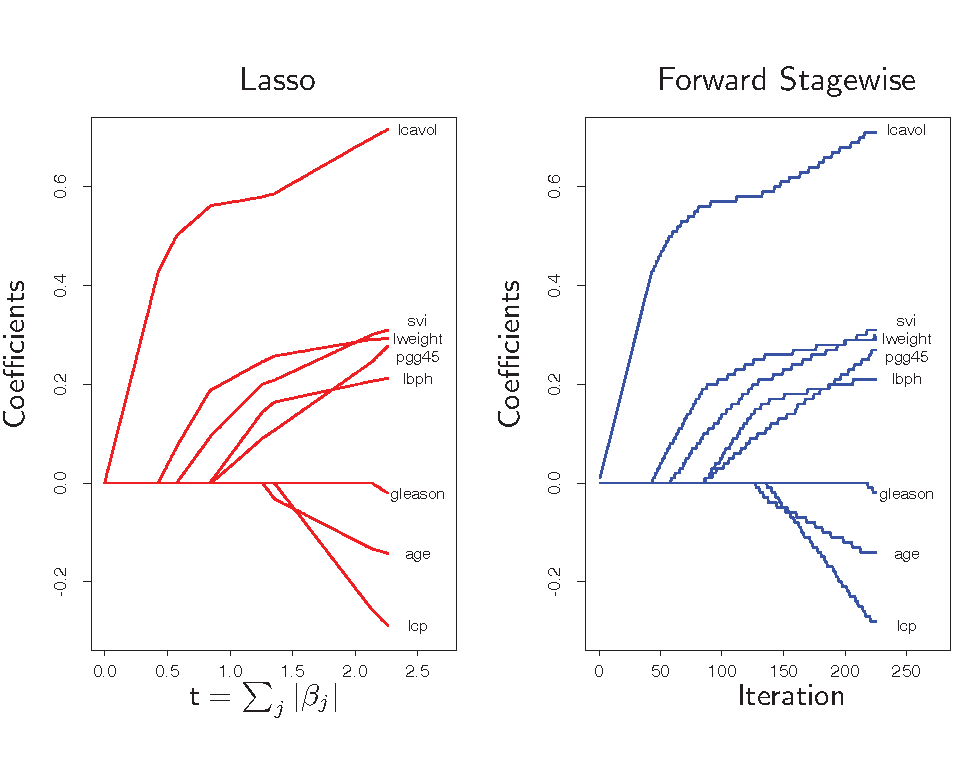
\includegraphics[width=0.8\textwidth]{identical.pdf}
\caption{左为Lasso, 右为Gradient Boosting} \label{fig1}
\end{figure}

后来Tibshirani找到自己的恩师Efron。Tibshirani在“\textit{The Science of Bradley Efron}”这本书的序言里写道,“\textit{\textbf{He sat down and pretty much single-handedly solved the problem. Along the way, he developed a new algorithm, `least angle regression', which is interesting in its own right, and sheds great statistical insight on the Lasso.}}” 我就不逐字逐句翻译了,大意是:Efron独自摆平了这个问题,与此同时发明了“Least Angle Regression (LAR)”。Efron结论是Lasso和Boosting的确有很紧密的数学联系,它们都可以通过修改LAR得到。更令人惊叹的是LAR具有非常明确的几何意义。于是,Tibshirani在序言中还有一句,“\textit{\textbf{In this work, Brad shows his great mathematical power–not the twentieth century, abstract kind of math, but the old-fashioned kind: geometric insight and analysis.}}” 读Prof Efron的文章,可以感受到古典几何学与现代统计学的结合之美(推荐大家读读Efron教授2010年的一本新书\textit{\textbf{Large-Scale Inference}},希望以后有机会再写写这方面的体会)!总之,Efron的这篇文章是现代统计学的里程碑,它结束了一个时代,开启了另一个时代。

这里,想补充说明一下Lasso的身世,它的全称是The Least Absolute Shrinkage and Selection Operator,读音不是[ `l\ae so]而是[l\ae' su:],有中文翻译为“套索”,个人觉得这个翻译不好,太远离它本来的含义,不如就用Lasso。Tibshrani自己说他的Lasso是受到Breiman的Non-Negative Garrote(NNG)的启发。 Lasso把NNG的两步合并为一步,即$L_1$-norm regularization。Lasso的巨大优势在于它所构造的模型是Sparse的,因为它会自动地选择很少一部分变量构造模型。现在,Lasso已经家喻户晓了,但是Lasso出生后的头两年却很少有人问津。后来Tibshirani自己回忆时说,可能是由下面几个原因造成的:1. 速度问题:当时计算机求解Lasso的速度太慢;2. 理解问题:大家对Lasso模型的性质理解不够(直到Efron的LAR出来后大家才搞明白);3. 需求问题:当时还没有遇到太多高维数据分析的问题,对Sparsity的需求似乎不足。Lasso的遭遇似乎在阐释我们已经熟知的一些道理: 1.千里马常有,而伯乐不常有(没有Efron的LAR,Lasso可能很难有这么大的影响力)。2. 时势造英雄(高维数据分析的问题越来越多,比如Bioinformatics领域)。3. 金子总是会闪光的。

LAR把Lasso($L_1$-norm regularization)和Boosting真正的联系起来,如同打通了任督二脉(数学细节可以参考本人的一个小结\footnote[1]{\url{http://ihome.ust.hk/~eeyang/lars_Lasso_boost.pdf}},当然最好还是亲自拜读Efron的原著)。LAR结束了一个晦涩的时代:在LAR之前,有关Sparsity的模型几乎都是一个黑箱,它们的数学性质(更不要谈古典的几何性质了)几乎都是缺失。LAR开启了一个光明的时代:有关Sparsity的好文章如雨后春笋般地涌现,比如Candes和Tao的Dantzig Selector。伯克利大学的Bin Yu教授称“\textit{Lasso, Boosting and Dantzig are three cousins}”。近年来兴起的Compressed Sensing(Candes \& Tao, Donoho)也与LAR一脉相承,只是更加强调$L_1$-norm regularization其他方面的数学性质,比如Exact Recovery。我觉得这是一个问题的多个方面,Lasso关注的是构建模型的准确性,Compressed Sensing关注的是变量选择的准确性。由此引起的关于Sparsity的研究,犹如黄河泛滥,一发不可收拾。比如Low-rank 逼近是把$L_1$-norm从向量到矩阵的自然推广(现在流行的“\textbf{用户推荐系统}”用到的Collaborative Filtering的数学原理源于此)。有兴趣的童鞋可以参考我个人的小结\footnote[2]{\url{http://ihome.ust.hk/~eeyang/Learning_from_sparsity.pdf}}。

还必须提到的是算法问题。我个人觉得,一个好的模型,如果没有一个快速准确的算法作为支撑的话,它最后可能什么也不是。看看Lasso头几年的冷遇就知道了。LAR的成功除了它漂亮的几何性质之外,还有它的快速算法。LAR的算法复杂度相当于最小二乘法的复杂度,这几乎已经把Lasso问题的求解推向极致。这一记录在2007年被Friedman的Coordinate Descent(CD)刷新,至今没人打破。Hastie教授趣称这个为“FFT(Friedman + Fortran + Tricks)”。因为CD对Generalized Lasso问题并不能一网打尽,许多凸优化解法应运而生,如Gradient Projection, Proximal methods,ADMM (Alternating Direction Method of Multipliers), (Split) Bregman methods,Nesterov's method (一阶梯度法中最优的收敛速度,Candes的很多软件包都根据这个方法设计) 等等。哪个方法更好呢?这个就像问“谁的武功天下第一”一样。我只能回答“王重阳以后再也没有天下第一了,东邪西毒南帝北丐,他们各有各的所长,有的功夫是这个人擅长一些,而另外几门功夫又是另一个人更擅长一些”。有关$L_1$的算法可能还会大量涌现,正如优化大师Stephen Boyd所说(2010年9月28日):“\textit{God knows the last thing we need is another algorithm for the Lasso}.”


\section{结语}
最后我想以讨论“模糊系统”和“统计学习”来结尾。这个话题非常具有争议,我就冒天下之大不讳吧,谈一谈我这几年的学习体会。记得十年前,立新老师曾经写过一篇文章《模糊系统:挑战与机遇并存——十年研究之感悟》,发表在2001年《自动化学报》上。我2005年看到的时候,敬仰之情,犹如滔滔江水。立新老师曾经有这么一句话:“\textit{If a method works well in practice, there must be some theoretical reasons for its success}.” 2005年的时候,我开始问自己什么使模糊系统的成功?立新老师认为有如下几个原因:1.模糊系统的通用逼近性能(Universal Approximator);2.模糊系统快速的构造算法,比如他自己的WM方法,Roger Jang的ANFIS等等;3.结果的可解释性;4.利用各种不同形式的信息。

下面我谈谈自己的看法,第一,通用逼近性能当然是一个好的性质,它表明模糊系统是很flexible的,但flexible的结构太多了,比如神经网络。问题往往不在flexible,而在太flexible导致overfitting。就如同SVM一样,没有$L_2$-norm regularization,实践中的性能就会变得很差。第二,快速算法,这是好的方法必备的,SVM,Boosting,Random Forest的算法都很快,而且可以直接用到高维,这一点上,我没有看到模糊系统的优势。第三,可解释性:模糊系统对低维数据(比如$2$ -- $4$维)的确具有好的解释性(因为IF-THEN规则的前提和结论都很简洁),但这个时候其它工具也可以做得到,比如Gradient Boosting和Random Forests(很多例子可以在ESL这本书里看到)。第四,充分的利用各种信息。立新老师指的是IF-THEN规则可以比较自由灵活的加入先验知识,并在他的书里面详细给出实例。遗憾的是,这些例子都在处理低维空间的问题。如何用IF-THEN规则解构高维空间呢?我个人看不到它们特殊的优势。然而,在统计学习里,利用不同的先验知识处理高维空间的例子比比皆是,比如Sparsity,group-structure,smoothness等等。现在举一个Gradient Boosting  Machine(GBM,也叫MART)的例子来说明我的观点。根据Lasso和Boosting的关系,可以知道GBM已经用到了Sparsity的性质($L_1$-norm regularization)。GBM有两个参数可以反映我们的先验知识。第一个参数是深度(depth),控制每棵决策树的深度 。如果深度为$1$,即树桩结构(Stump),表明GBM将采用加法模型(Generalized Additive Model),即不考虑变量之间的交互式作用(Interaction);如果深度大于$1$,则考虑交互式作用。因为交互式作用在非线性建模中比较重要,如异或(XOR)问题,没有考虑交互式作用将失败得很惨,所以这个参数设置反映了对非线性建模的先验。第二个参数是Shrinkage的大小。假设深度选取是合理的,在噪声比较小的时候,没有Shrinkage会比较好;噪声比较大的时候,有Shrinkage会好一些。实践中,使用GBM对高维数据分析,试错法(Trial and Error)很容易使用,因为就这两个参数(通常$\text{depth} = 3 \text{~} 4$;实际数据的噪声往往比较大,推荐设置$\text{Shrinkage} = 0.01$)。模型构建好之后,GBM会告诉你哪些变量是重要的,变量之间的交互式作用如何等等,这样模型的结果也是比较容易理解。Random Forests也有相似的功能。好了,最后借Hastie教授的一幅图来总结一下,无疑,GBM(MART)是他们的最爱,也是我的最爱。

\begin{figure}[htbp]
\centering
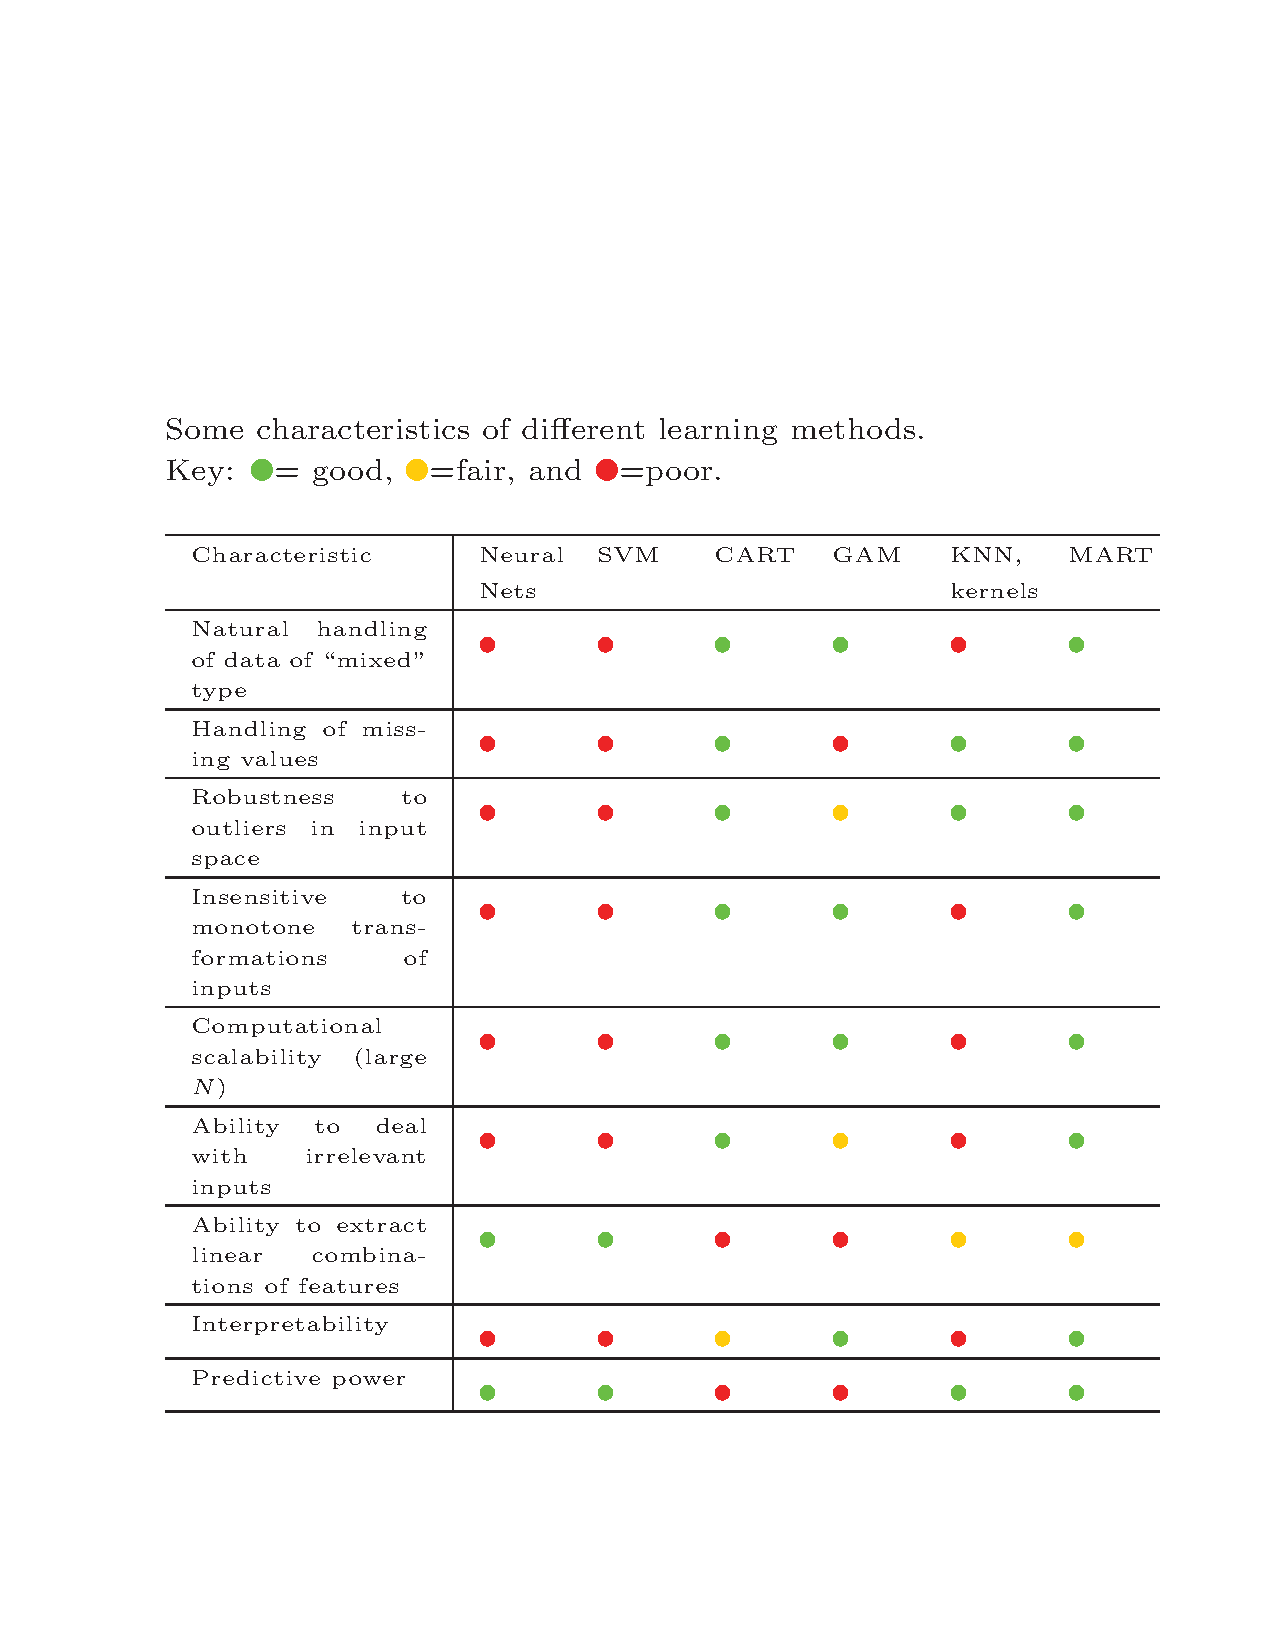
\includegraphics[width=0.75\textwidth]{compare.pdf}
\caption{各类学习方法的特性总结} \label{fig2}
\end{figure}

\section*{尾音}
\begin{quote}
\begin{itemize}

\item 问:世间是否此山最高,或者另有高处比天高?

\item 答: 在世间自有山比此山更高,Open-mind要比天高。
\end{itemize}
\end{quote}
\end{document}
